% Search for all the places that say "PUT SOMETHING HERE".

\documentclass[11pt]{article}
\usepackage{amsmath,textcomp,amssymb,graphicx,enumerate,hyperref,enumitem,mathtools,tikz-qtree,listings,tikz}

\def\Name{Jonathan Sun}  % Your name
\def\SID{25020651}  % Your student ID number
\def\Homework{3} % Number of Homework
\def\Session{Fall 2017}


\title{CS170 --- \Session --- Homework \Homework \space Solutions}
\author{\Name, SID \SID}
\markboth{CS170 --- \Session --- Homework \Homework \space --- \Name}{CS170 --- \Session --- Homework \Homework --- \Name}
\pagestyle{myheadings}
\date{}

\def\endproofmark{$\Box$}
\newenvironment{proof}{\par{\bf Proof:}}{\endproofmark\smallskip}
\newenvironment{FourPartSolution}{\par{\bf Four-Part Solution:}}{\smallskip}
\newenvironment{mainIdea}{{\bf Main Idea:}}{\smallskip}
\newenvironment{pseudocode}{\par{\bf Pseudocode:}}{\smallskip}
\newenvironment{proofOfCorrectness}{\par{\bf Proof of Correctness:}}{\endproofmark\smallskip}
\newenvironment{runTime}{{\bf Run Time:}}{\smallskip}
\newenvironment{justification}{\par{\bf Justification:}}{\smallskip}
% \newenvironment{proofOfCorrectness}{\par{\bf Proof of Correctness:}}{\endproofmark\smallskip}
% \newenvironment{runTime}{\par{\bf Run Time:}}{\smallskip}
% \newenvironment{justification}{\par{\bf Justification:}}{\smallskip}

\usepackage[margin=1in]{geometry}



\begin{document}
\maketitle

\section*{0. Who Did You Work With?}

Collaborators: Kevin Vo, Aleem Zaki, Jeremy Ou



\newpage
\section*{1. Minimal Positive Valued Function}
\begin{mainIdea}
\\
ok
\end{mainIdea}
\\
\begin{runTime}
\\
ok
\end{runTime}


\newpage
\section*{2. Graph Basics}
\begin{enumerate}[label=(\alph*)]
\item
Yes. The algorithm to find the shortest path between $s$ and $t$ may have terminated before hitting $t'$ or $t'$ was never going to be hit in the first place when going from $s$ to $t'$.

\item
No. The algorithm will not be guaranteed to return the same solution because of the following counterexample:
\vspace*{1\baselineskip}
\\
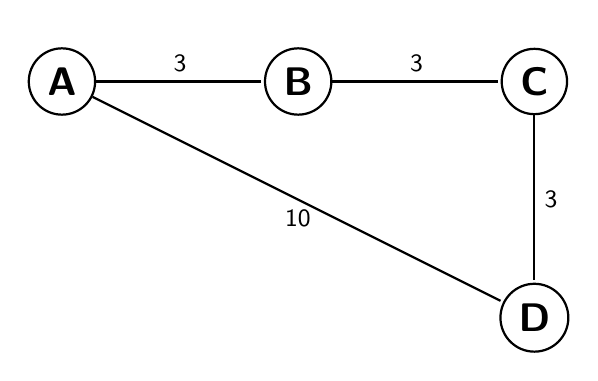
\begin{tikzpicture}[shorten >=1pt, auto, node distance=3cm, thick, main node/.style={circle, draw, font=\sffamily\Large\bfseries}]
	\node[main node, label] (A) {A};
	\node[main node, label] (B) [right of=A] {B};
	\node[main node, label] (C) [right of=B] {C};
	\node[main node, label] (D) [below of=C] {D};

	\path[every node/.style={font=\sffamily\small}]
		(A) edge node [above] {3} (B)
			edge node [below] {10} (D)
		(B) edge node [above] {3} (C)
		(C) edge node [right] {3} (D);
\end{tikzpicture}
\\
Running Dijkstra's algorithm from $A$ to $D$ will return $A$, $B$, $C$, $D$. However, adding $5$ to the lengths of all edges gives us:
\\
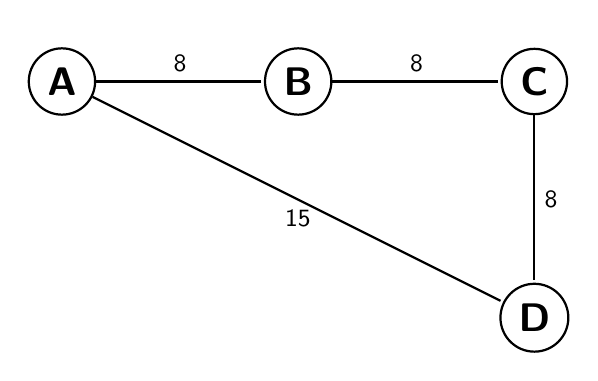
\begin{tikzpicture}[shorten >=1pt, auto, node distance=3cm, thick, main node/.style={circle, draw, font=\sffamily\Large\bfseries}]
	\node[main node, label] (A) {A};
	\node[main node, label] (B) [right of=A] {B};
	\node[main node, label] (C) [right of=B] {C};
	\node[main node, label] (D) [below of=C] {D};

	\path[every node/.style={font=\sffamily\small}]
		(A) edge node [above] {8} (B)
			edge node [below] {15} (D)
		(B) edge node [above] {8} (C)
		(C) edge node [right] {8} (D);
\end{tikzpicture}
\\
Running Dijkstra's algorithm from $A$ to $D$ will return $A$, $D$ instead of $A$, $B$, $C$, $D$.

\item
No. If an edge length becomes negative, then Dijkstra’s algorithm will not work.

\item
Yes.

\end{enumerate}



\newpage
\section*{3. Peak Element}




\newpage
\section*{4. Exact Change}




\newpage
\section*{5. Local Maxima}




\newpage
\section*{6. DNA Sequence Alignment}


\end{document}
